%\documentclass[]{article}
\documentclass[11pt]{article}
\usepackage[usenames,dvipsnames]{xcolor}

\usepackage[T1]{fontenc}
%\usepackage{lmodern}
\usepackage{tgtermes}
\usepackage{amssymb,amsmath}
%\usepackage[margin=1in]{geometry}
\usepackage[letterpaper,bottom=1in,top=1in,right=1in,left=1in,includemp=FALSE]{geometry}
\usepackage{pdfpages}
\usepackage[small,labelfont=bf]{caption}
\usepackage{subcaption}
\usepackage{multirow}
\usepackage{longtable}
\usepackage{pdflscape}
\usepackage{array}
\usepackage{amssymb}
\usepackage{graphicx}

\newcolumntype{P}[1]{>{\raggedright\arraybackslash}p{#1}}
\usepackage{tikz}
\usetikzlibrary{mindmap, positioning}


\usepackage{ifxetex,ifluatex}
\usepackage{fixltx2e} % provides \textsubscript
% use microtype if available
\IfFileExists{microtype.sty}{\usepackage{microtype}}{}
\ifnum 0\ifxetex 1\fi\ifluatex 1\fi=0 % if pdftex
\usepackage[utf8]{inputenc}
\else % if luatex or xelatex
\usepackage{fontspec}
\ifxetex
\usepackage{xltxtra,xunicode}
\fi
\defaultfontfeatures{Mapping=tex-text,Scale=MatchLowercase}
\newcommand{\euro}{€}
\fi
%

\usepackage{fancyvrb}

\usepackage{ctable,longtable}

\usepackage{float} % provides the H option for float placement
\usepackage{dcolumn} % allows for different column alignments
\newcolumntype{.}{D{.}{.}{1.2}}

\usepackage{booktabs} % nicer horizontal rules in tables

%Assume we want graphics always
\usepackage{graphicx}
% We will generate all images so they have a width \maxwidth. This means
% that they will get their normal width if they fit onto the page, but
% are scaled down if they would overflow the margins.
%% \makeatletter
%% \def\maxwidth{\ifdim\Gin@nat@width>\linewidth\linewidth
%%   \else\Gin@nat@width\fi}
%% \makeatother
%% \let\Oldincludegraphics\includegraphics
%% \renewcommand{\includegraphics}[1]{\Oldincludegraphics[width=\maxwidth]{#1}}
\graphicspath{{.}}


%% \ifxetex
%% \usepackage[pagebackref=true, setpagesize=false, % page size defined by xetex
%% unicode=false, % unicode breaks when used with xetex
%% xetex]{hyperref}
%% \else
\usepackage[pagebackref=true, unicode=true, bookmarks=true, pdftex]{hyperref}
% \fi


\hypersetup{breaklinks=true,
  bookmarks=true,
  pdfauthor={Christopher Grady, Rebecca Wolfe, Danjuma Dawop, and Lisa Inks},
  pdftitle={Promoting Peace Amid Intergroup Conflict: An Intergroup Contact Field Experiment in Nigeria},
  pdfkeywords = {group conflict, intergroup contact, Nigeria, field
experiment},
  colorlinks=true,
  linkcolor=BrickRed,
  citecolor=blue, %MidnightBlue,
  urlcolor=BrickRed,
  % urlcolor=blue,
  % linkcolor=magenta,
  pdfborder={0 0 0}}

%\setlength{\parindent}{0pt}
%\setlength{\parskip}{6pt plus 2pt minus 1pt}
%\usepackage{parskip}
\setlength{\emergencystretch}{3em}  % prevent overfull lines
\providecommand{\tightlist}{%
  \setlength{\itemsep}{0pt}\setlength{\parskip}{0pt}}

%% Insist on this.
\setcounter{secnumdepth}{2}

\VerbatimFootnotes % allows verbatim text in footnotes

\title{Promoting Peace Amid Intergroup Conflict: An Intergroup Contact
Field Experiment in Nigeria}

\author{\parbox{.7\linewidth}{\centering
Christopher Grady, Rebecca Wolfe, Danjuma Dawop, and Lisa Inks
}
}

\date{October 14, 2020}

\usepackage{versions}
\makeatletter
\renewcommand*\versionmessage[2]{\typeout{*** `#1' #2. ***}}
\renewcommand*\beginmarkversion{\sffamily}
  \renewcommand*\endmarkversion{}
\makeatother

\excludeversion{comment}

%\usepackage[margins=1in]{geometry}

\usepackage[compact,bottomtitles]{titlesec}
\setcounter{secnumdepth}{3}
%\titleformat{ ⟨command⟩}[⟨shape⟩]{⟨format⟩}{⟨label⟩}{⟨sep⟩}{⟨before⟩}[⟨after⟩]
\titleformat{\section}[hang]{\Large\bfseries}{\thesection}{.5em}{\hspace{0in}}[\vspace{-.2\baselineskip}]
\titleformat{\subsection}[hang]{\large\bfseries}{\thesubsection}{.5em}{\hspace{0in}}[\vspace{-.2\baselineskip}]
\titleformat{\subsubsection}[hang]{\bfseries}{\thesubsubsection}{.5em}{\hspace{0in}}[\vspace{-.2\baselineskip}]
%\titleformat{\subsubsection}[runin]{\bfseries}{\thesubsubsection}{1ex}{}[\vspace{-.2\baselineskip}]
\titleformat{\paragraph}[runin]{\bfseries\itshape}{\theparagraph}{1ex}{}{\vspace{-.2\baselineskip}}
%\titleformat{\paragraph}[runin]{\itshape}{\theparagraph}{1ex}{}{\vspace{-.2\baselineskip}}

%%\titleformat{\subsection}[hang]{\bfseries}{\thesubsection}{.5em}{\hspace{0in}}[\vspace{-.2\baselineskip}]
%%%\titleformat*{\subsection}{\bfseries\scshape}
%%%\titleformat{\subsubsection}[leftmargin]{\footnotesize\filleft}{\thesubsubsection}{.5em}{}{}
%%\titleformat{\subsubsection}[hang]{\small\bfseries}{\thesubsubsection}{.5em}{\hspace{0in}}[\vspace{-.2\baselineskip}]
%%\titleformat{\paragraph}[runin]{\itshape}{\theparagraph}{1ex}{}{\vspace{-.5\baselineskip}}

%\titlespacing*{ ⟨command⟩}{⟨left⟩}{⟨beforesep⟩}{⟨aftersep⟩}[⟨right⟩]
\titlespacing{\section}{0pc}{1.5ex plus .1ex minus .2ex}{.5ex plus .1ex minus .1ex}
\titlespacing{\subsection}{0pc}{1.5ex plus .1ex minus .2ex}{.5ex plus .1ex minus .1ex}
\titlespacing{\subsubsection}{0pc}{1.5ex plus .1ex minus .2ex}{.5ex plus .1ex minus .1ex}



%% These next lines tell latex that it is ok to have a single graphic
%% taking up most of a page, and they also decrease the space around
%% figures and tables.
\renewcommand\floatpagefraction{.9}
\renewcommand\topfraction{.9}
\renewcommand\bottomfraction{.9}
\renewcommand\textfraction{.1}
\setcounter{totalnumber}{50}
\setcounter{topnumber}{50}
\setcounter{bottomnumber}{50}
\setlength{\intextsep}{2ex}
\setlength{\floatsep}{2ex}
\setlength{\textfloatsep}{2ex}

\usepackage{setspace}
\doublespacing
\setlength{\parindent}{4em}

\begin{document}
\VerbatimFootnotes

%\begin{titlepage}
%  \maketitle
%\vspace{2in}
%
%\begin{center}
%  \begin{large}
%    PROPOSAL WHITE PAPER
%
%BAA 14-013
%
%Can a Hausa Language Television Station Change Norms about Violence in Northern Nigeria? A Randomized Study of Media Effects on Violent Extremism
%
%Jake Bowers
%
%University of Illinois @ Urbana-Champaign (jwbowers@illinois.edu)
%
%\url{http://jakebowers.org}
%
%Phone: +12179792179
%
%Topic Number: 1
%
%Topic Title: Identity, Influence and Mobilization
%
%\end{large}
%\end{center}
%\end{titlepage}

\newlength{\cslhangindent}
\setlength{\cslhangindent}{1.5em}
\newenvironment{cslreferences}%
  {\setlength{\parindent}{0pt}%
  \everypar{\setlength{\hangindent}{\cslhangindent}}\ignorespaces}%
  {\par}

\maketitle


\newcommand\blfootnote[1]{%
  \begingroup
  \renewcommand\thefootnote{}\footnote{#1}%
  \addtocounter{footnote}{-1}%
  \endgroup
}
\singlespacing\blfootnote{Thanks to Jake Bowers, Jim Kuklinski, Justin
Rhodes, Cara Wong, Caglayan Baser, Ekrem Baser, Nuole Chen, Alice
Iannantuoni, Betsy Rajala, Charla Waeiss, and Donald Beaudette for
useful conversations and feedback on the many drafts of this paper.
Thanks to the Mercy Corps Nigeria team for their work implementing the
peacebuilding project. Thanks to Tahiru Ahmadu, Ibrahim Hassan, and the
enumeration teams for their excellent work interviewing farmers and
pastoralists. Thanks to Hadiza Nuhu and Israel Okpe for their work as
the main contact people and mobilizers in farming and pastoral
communities. Thanks to the participants in the Evidence in Governance
and Politics 2015 workshop at Rice University for design input.}

\hypertarget{appendices}{%
\section{Appendices}\label{appendices}}

\hypertarget{appendix-a-randomization-inference-and-bootstrapping}{%
\subsection{Appendix A: Randomization Inference and
Bootstrapping}\label{appendix-a-randomization-inference-and-bootstrapping}}

Randomization inference and bootstrapping are nonparametric methods to
generate \(p\)-values (randomization inference) and confidence intervals
(bootstrapping). With \emph{randomization inference}, we first shuffle
the treatment variable to break the relationship between treatment and
outcomes. Next we regress outcomes on treatment using our regression
equation and store the resulting coefficient. Lastly, we repeat that
process 10,000 times to create the distribution of coefficients we would
observe if treatment had no effect on outcomes -- the null hypothesis.
Our \(p\)-value is the proportion of the null distribution that is
greater than or equal to our observed coefficient.

\emph{Bootstrapping} for standard errors is similar, but instead of
shuffling the treatment indicator we resample units with replacement. By
resampling with replacement, we create the empirical distribution of our
data and the range of possible treatment effects we might observe if we
repeated the experiment 10,000 times. The treatment effect at the 2.5th
percentile and at the 97.5th percentile are equivalent to a 95\%
confidence interval (Efron and Tibshirani 1994).

In each of these procedures, we mimic our randomization process by
randomizing/resampling the intervention to communities in site-level
clusters and within state blocks. This means that both communities in an
implementation site (farmers and pastoralists) will always be
treated/sampled together and that assignment to the intervention and
resampling are conducted separately in Nassarawa and Benue, just as the
intervention was assigned in this study. This procedure ensures that our
null distribution (for \(p\)-values) is created by randomizing the
intervention between exchangeable units and that our empirical
distribution (for confidence intervals) is created by resampling units
as they were sampled.

\hypertarget{appendix-b-results-with-additive-indices}{%
\subsection{Appendix B: Results with Additive
Indices}\label{appendix-b-results-with-additive-indices}}

These tables show results for self-report survey outcomes made with
additive indices. The tables include the coefficients and \(p\)-values
with additive indices for community- and individual-level analyses.

\begin{table}[H]
\begin{center}

\begin{tabular}{l|r|r|r|r}
\hline
  & ag\_coef & ag\_p & ind\_coef & ind\_p\\
\hline
Affect & 0.093 & 0.037 & 0.062 & 0.056\\
\hline
Insecurity & 0.015 & 0.174 & 0.030 & 0.011\\
\hline
Contact & 0.054 & 0.193 & 0.070 & 0.143\\
\hline
\end{tabular}


\caption{\label{tab:add_ind_tab}\textbf{Effect of the intervention on main outcomes with additive indices.} The first and second columns are coefficients and $p$-values for aggregate community-level analyses.  The third and fourth columns are coefficients and $p$-values for individual-level analyses.}
\end{center}
\end{table}

\hypertarget{appendix-c-mechanisms-and-placebo-analysis}{%
\subsection{Appendix C: Mechanisms and Placebo
Analysis}\label{appendix-c-mechanisms-and-placebo-analysis}}

These tables show results for mechanism and placebo outcomes using
inverse-covariance weighted indices. The tables include the coefficients
and \(p\)-values for community- and individual-level analyses.

\begin{table}[H]
\begin{center}

\begin{tabular}{l|r|r|r|r}
\hline
  & ag\_coef & ag\_p & ind\_coef & ind\_p\\
\hline
Threat & -0.065 & 0.796 & 0.007 & 0.350\\
\hline
Empathy & 0.129 & 0.089 & 0.127 & 0.010\\
\hline
Perspective-Taking & -0.040 & 0.640 & 0.029 & 0.195\\
\hline
Ingroup Expansion & 0.036 & 0.252 & 0.016 & 0.166\\
\hline
Placebo (Violence) & -0.067 & 0.691 & -0.007 & 0.556\\
\hline
\end{tabular}


\caption{\label{tab:mech_ind_tab}\textbf{Effect of the intervention on mechanism and placebo outcomes.} The first and second columns are coefficients and $p$-values for aggregate community-level analyses.  The third and fourth columns are coefficients and $p$-values for individual-level analyses.}
\end{center}
\end{table}

Plots for the social desirability check/placebo outcome are presented in
Figures \ref{fig:vio_comm} and \ref{fig:vio_ind}.

\begin{figure}[H]
    \begin{subfigure}[b]{.48\textwidth}
    \centering
        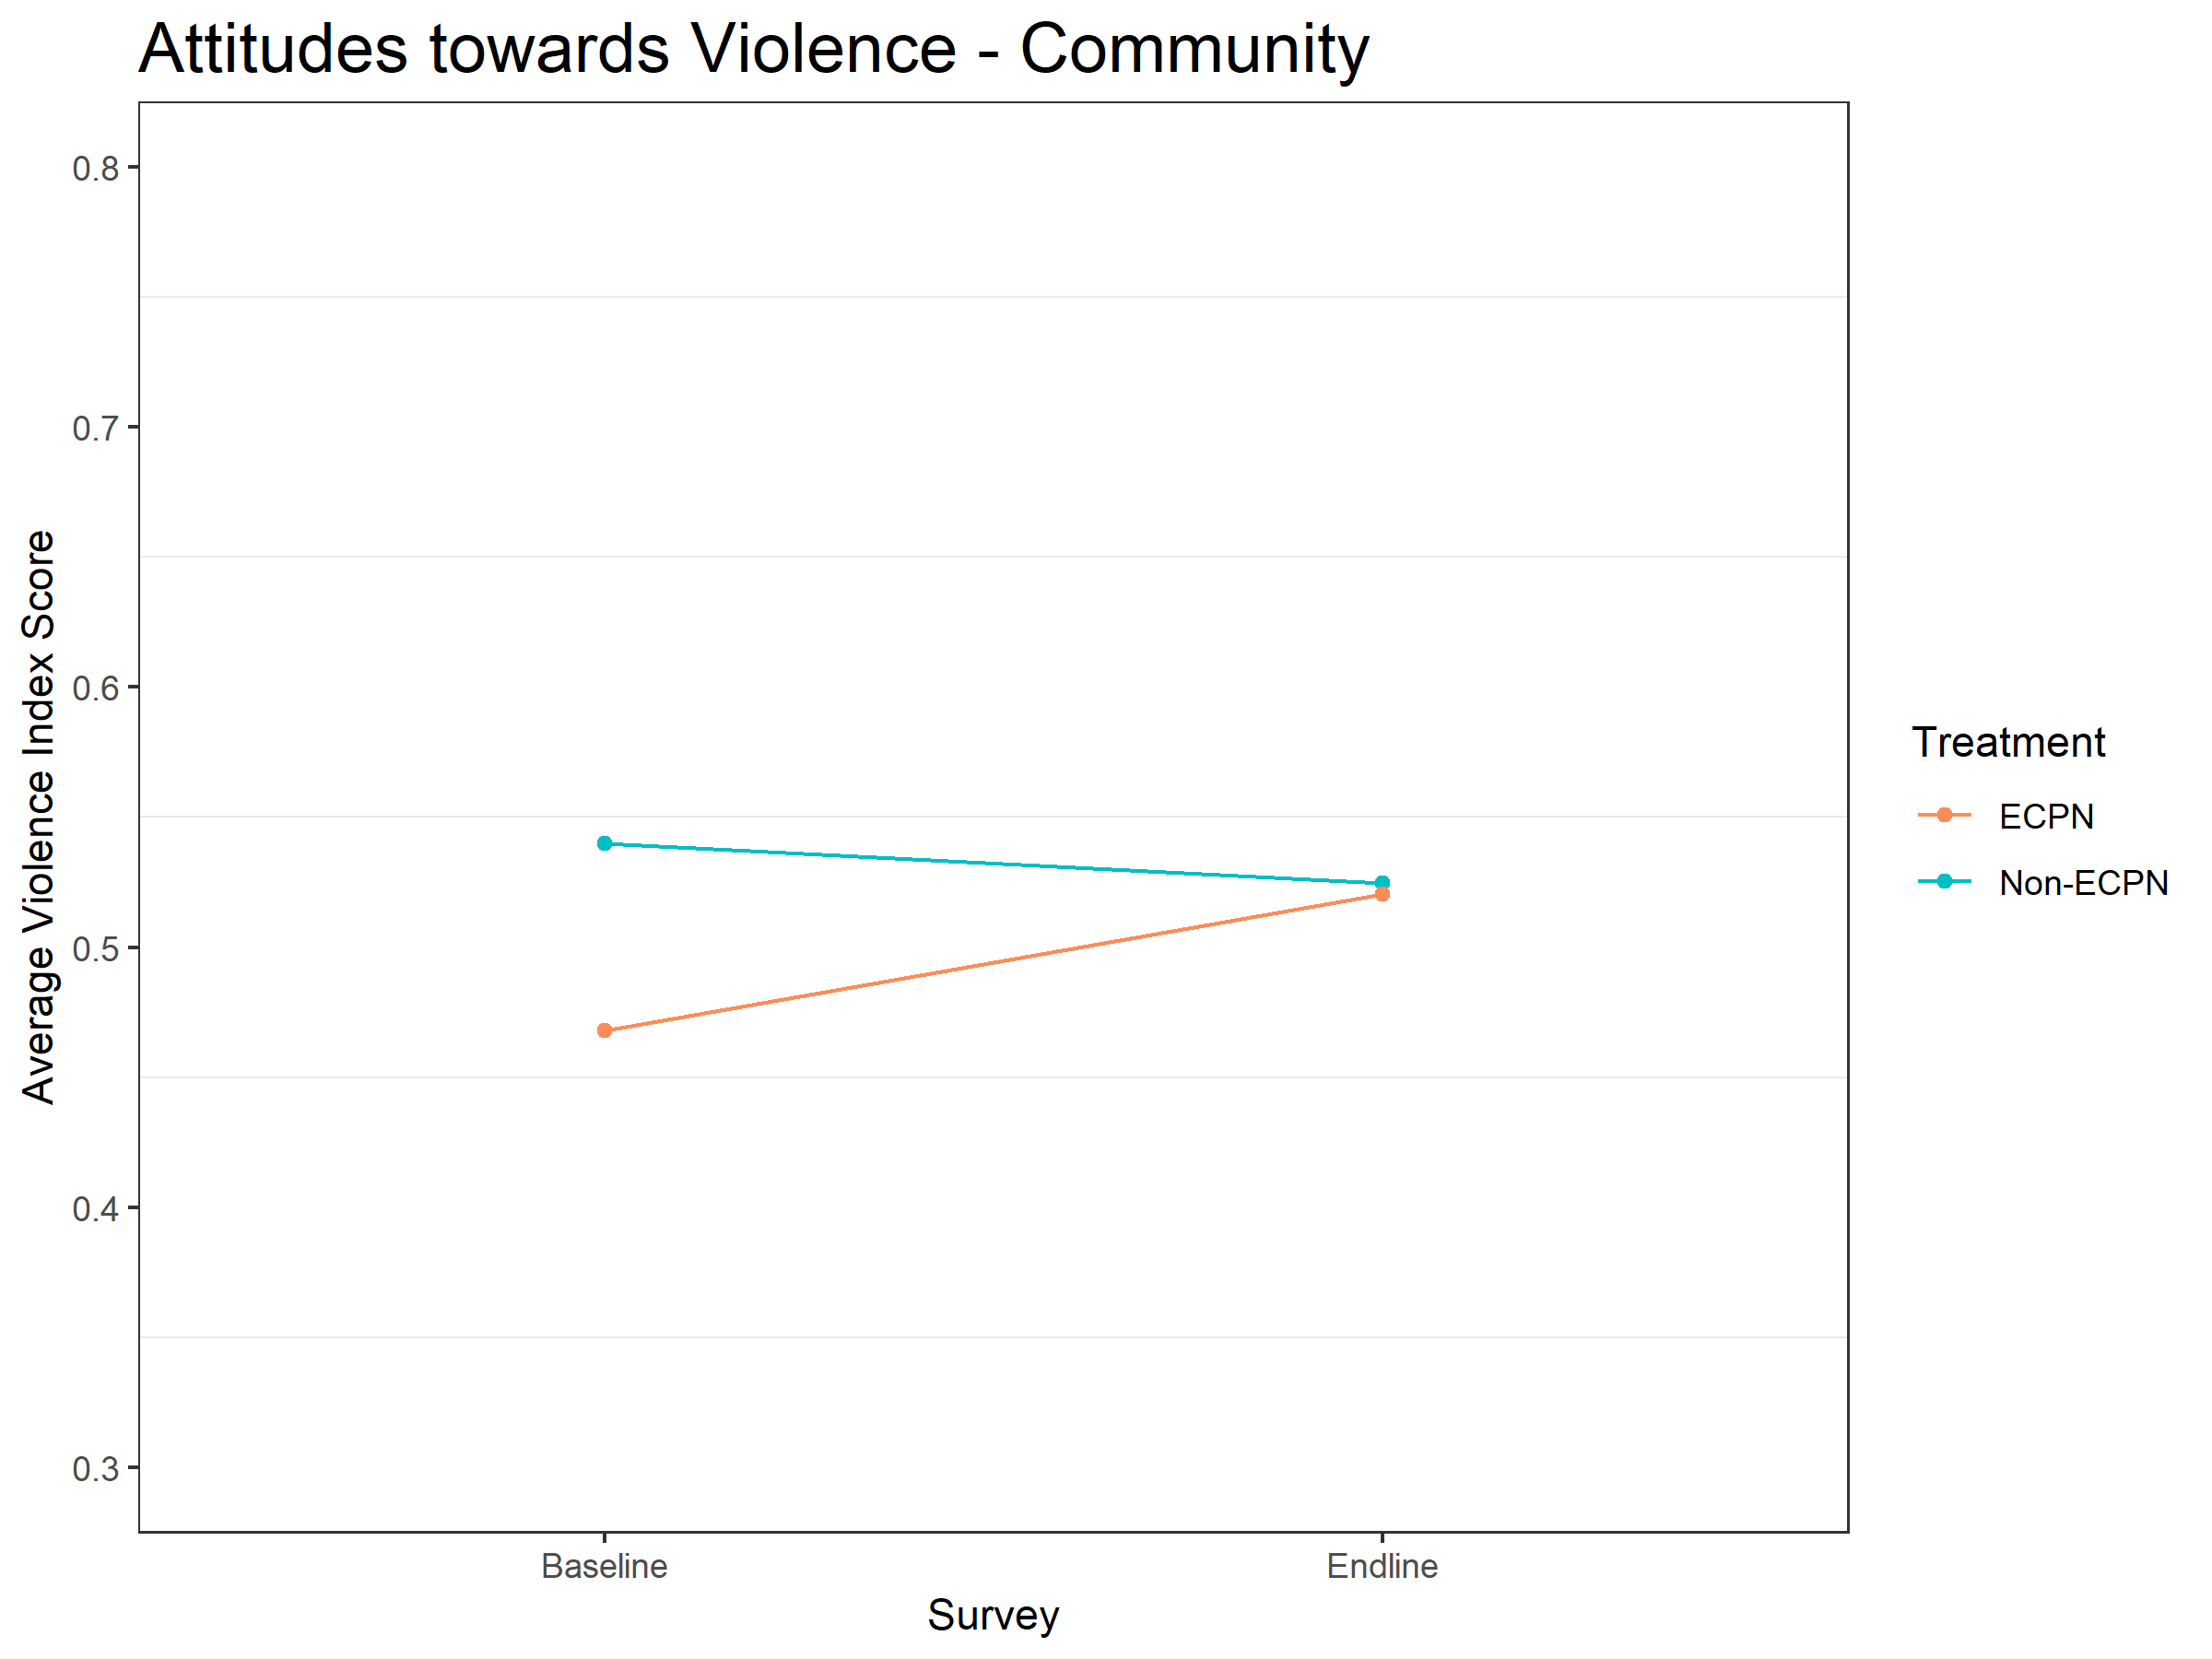
\includegraphics[width=\linewidth]{../../../figs/vioComm_plot.png}
        \caption{\textbf{Descriptive change in community-level attitudes towards violence from baseline to endline.} Red line is treatment site average, blue line is control site average.}
        \label{fig:vio_comm}
    \end{subfigure}
    \hfill
    \begin{subfigure}[b]{.48\textwidth}
    \centering
        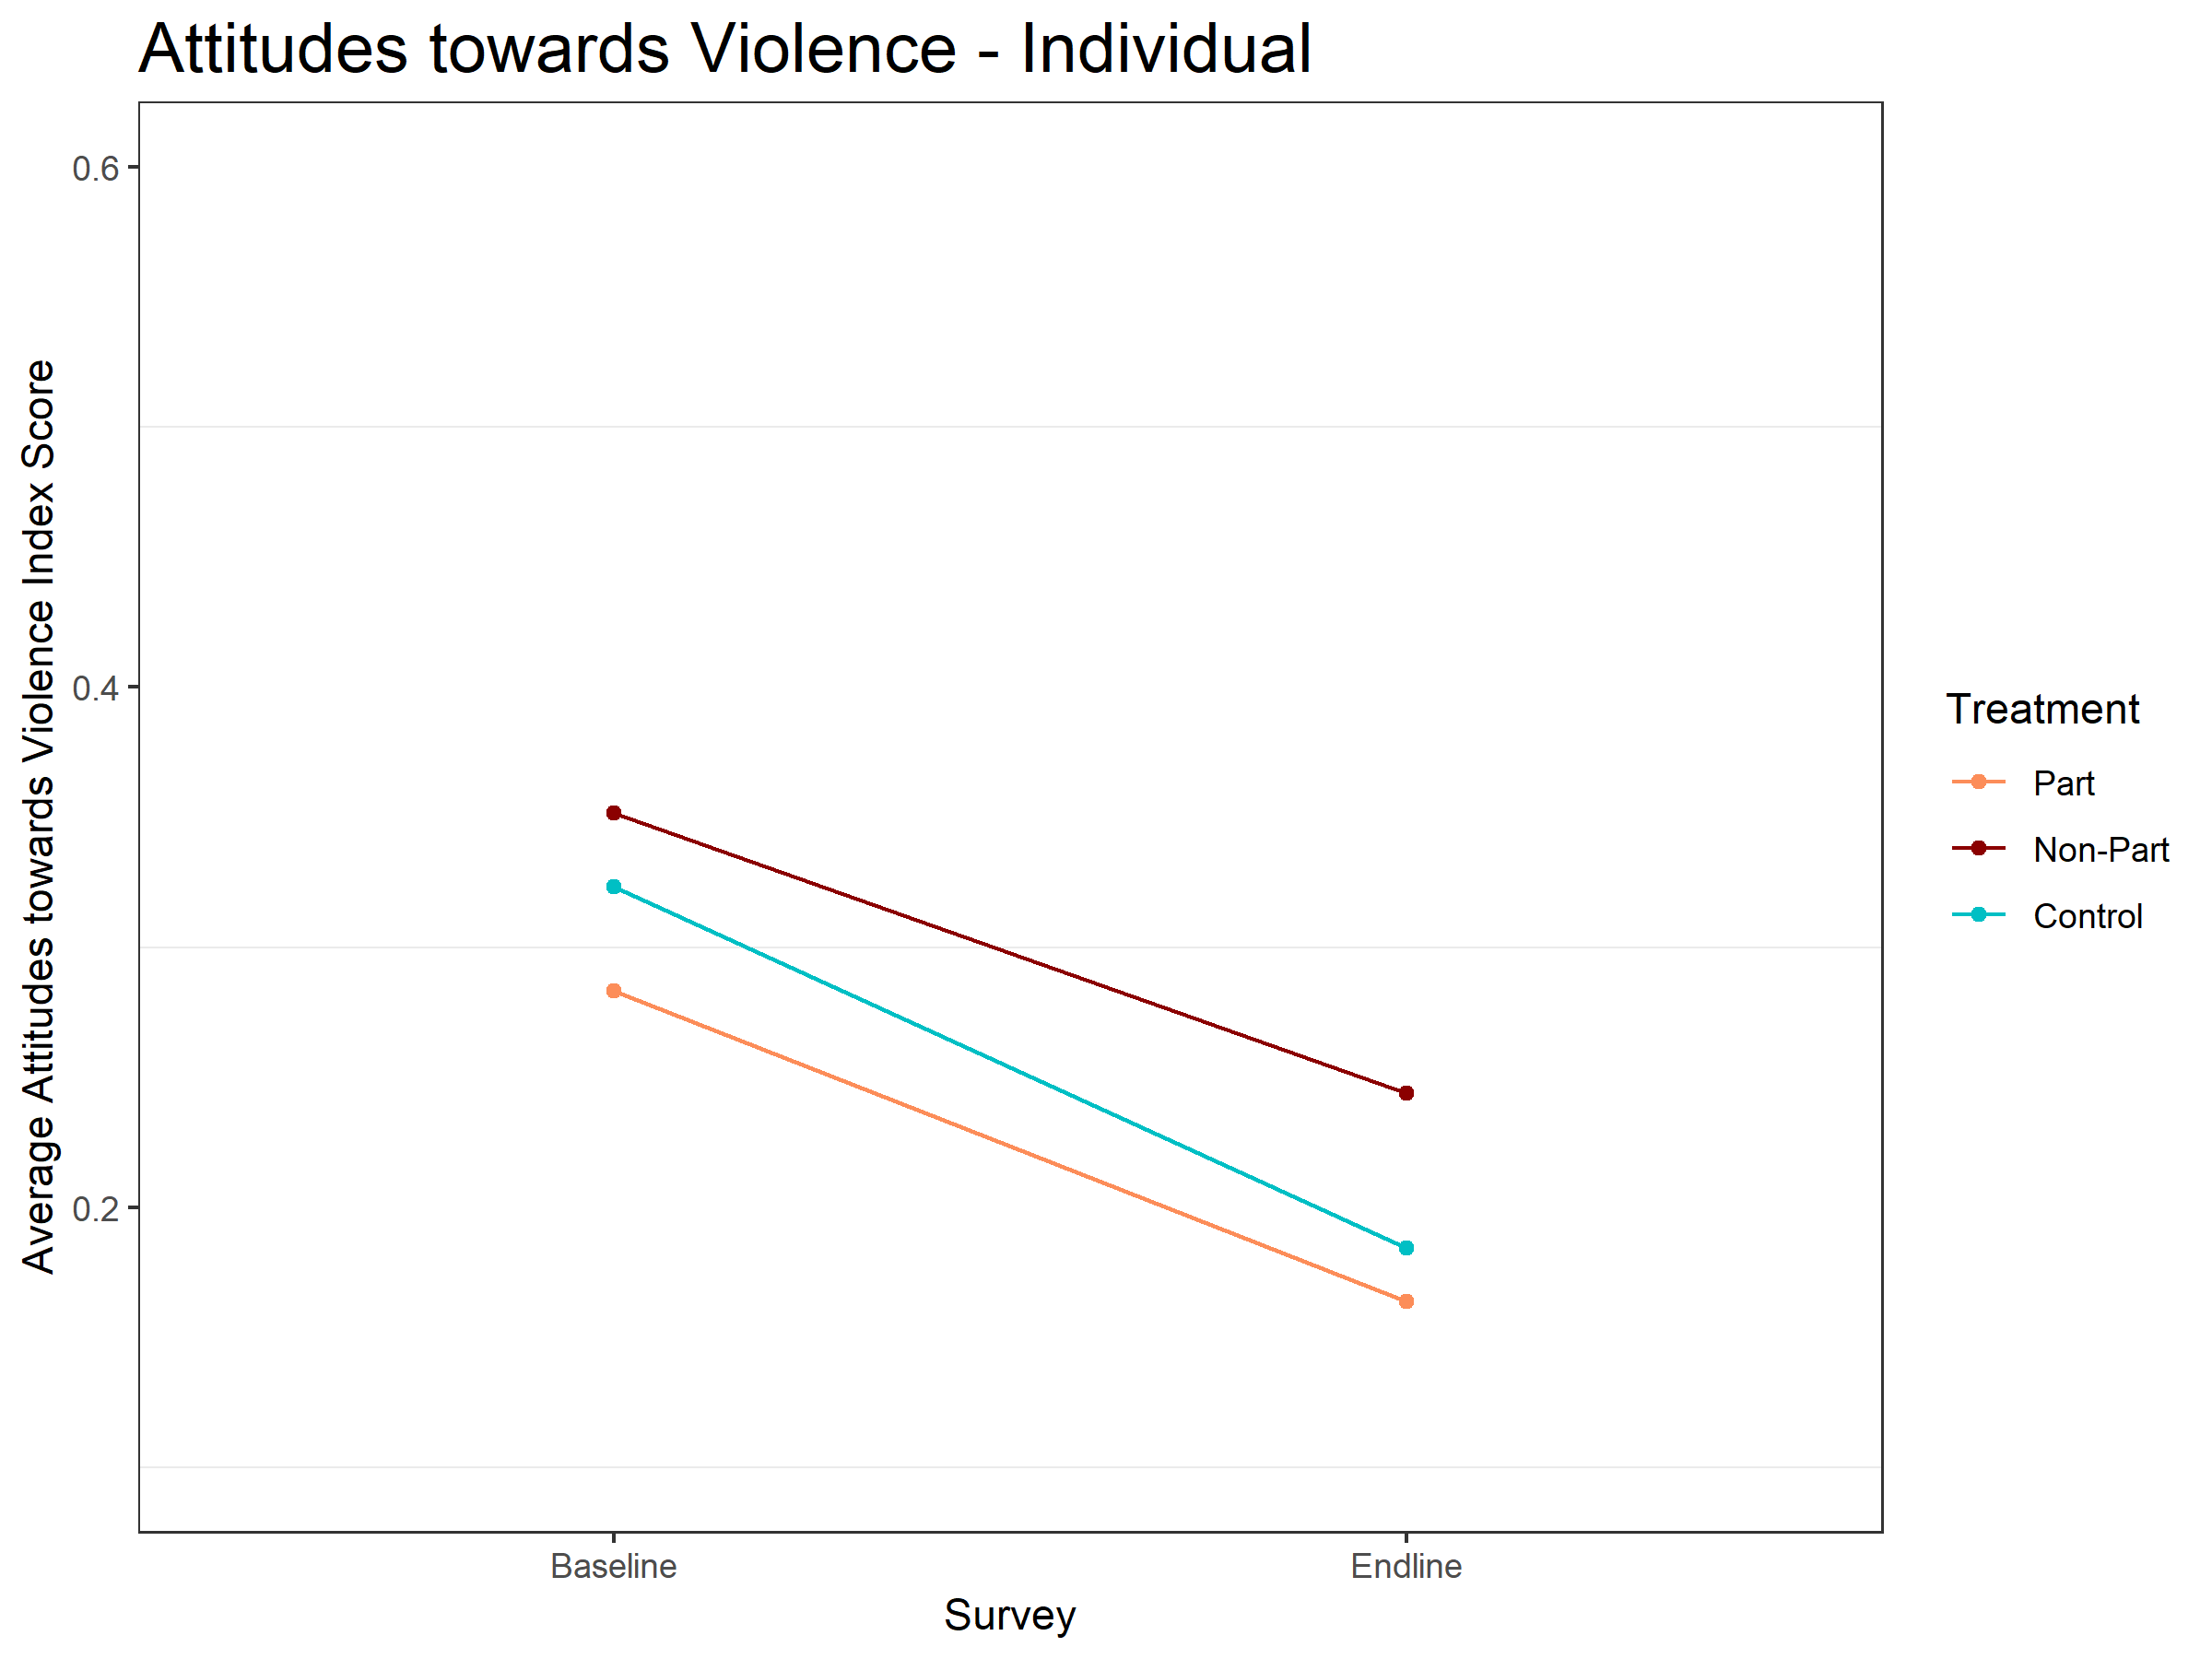
\includegraphics[width=\linewidth]{../../../figs/vioPan_plot.png}
        \caption{\textbf{Descriptive change in individual-level attitudes towards violence from baseline to endline.} Red line is participant average, dark red line is nonparticipant average, blue line is control average.}
        \label{fig:vio_ind}
    \end{subfigure}
    \caption{\textbf{Social desirability check: attitudes towards violence.}  Moving up the Y-axis indicates more acceptance of violence.}
\end{figure}

\hypertarget{appendix-d-endorsement-exp-plot}{%
\subsection{Appendix D: Endorsement Exp
Plot}\label{appendix-d-endorsement-exp-plot}}

Figure \ref{fig:end1} shows the descriptive results of the endorsement
experiment.

\begin{figure}[H]
\centering
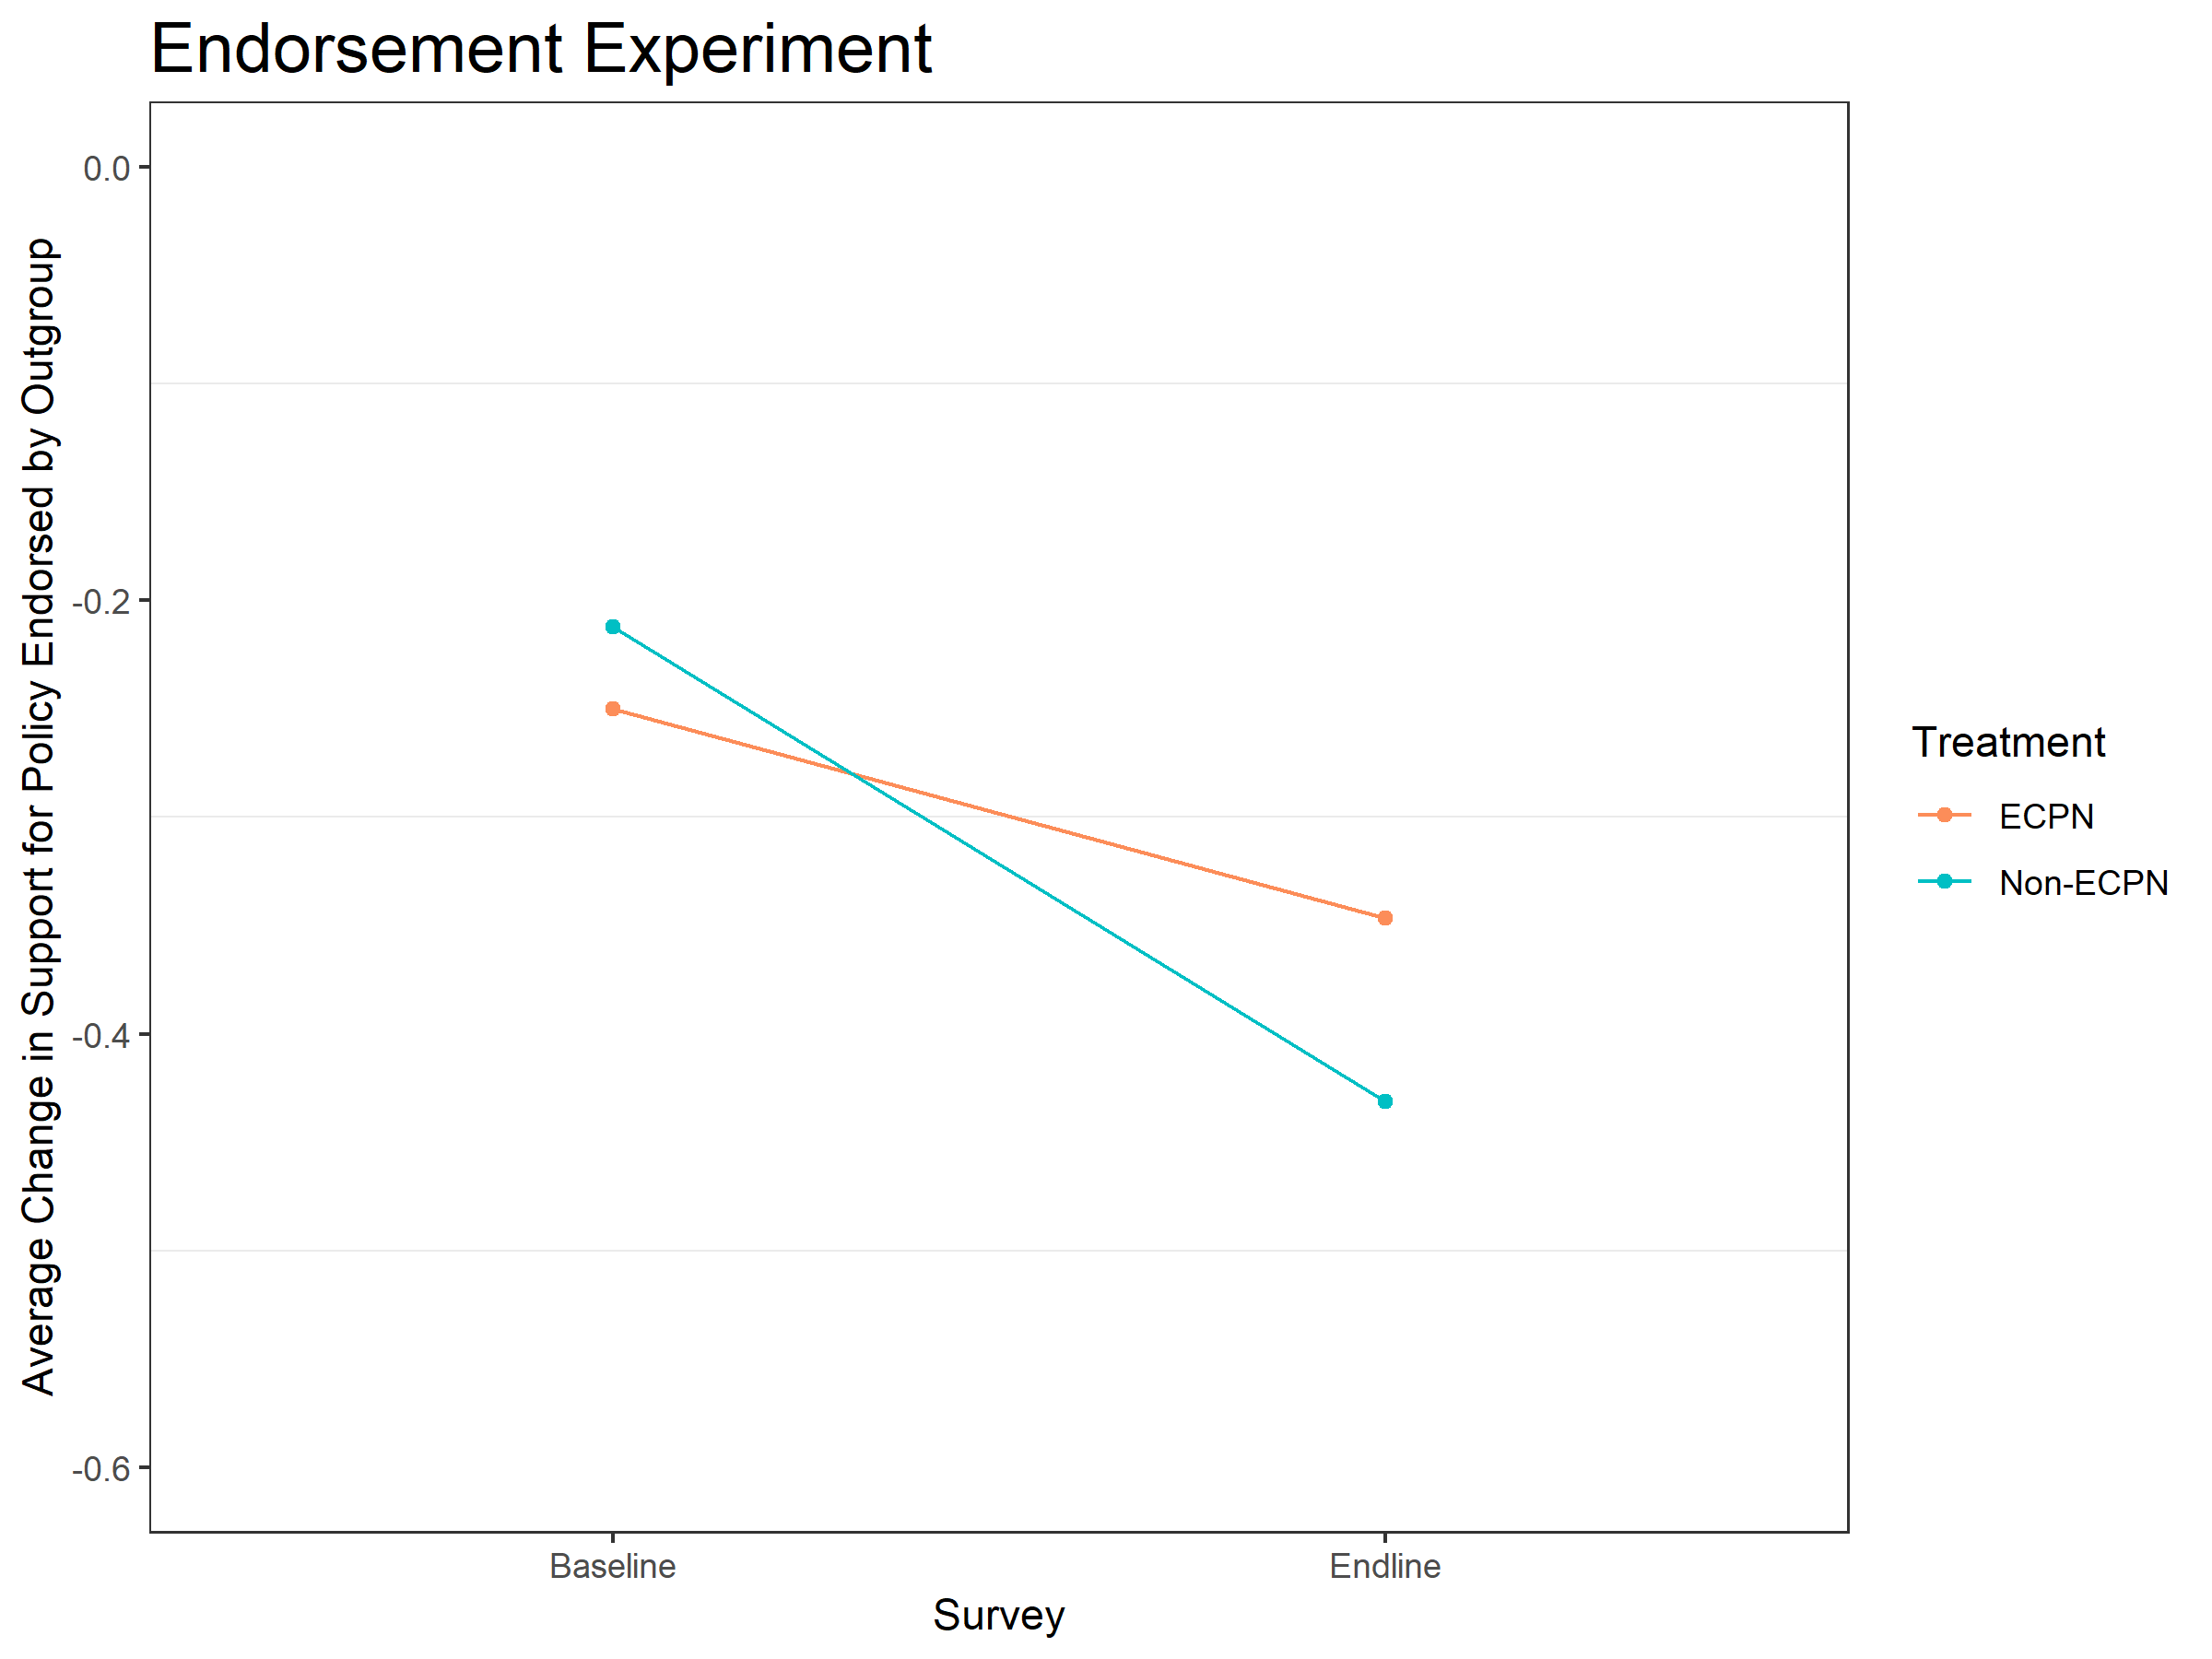
\includegraphics[width=.7\textwidth]{../../../figs/endComm_plot.png}
\caption{\label{fig:end1} \textbf{Effect of outgroup endorsement on policy support for treatment and control sites.} Red line is treatment site average, blue line is control site average.  Moving down the Y-axis indicates decreased trust in other group.}
\end{figure}

\hypertarget{appendix-e-survey-questions}{%
\subsection{Appendix E: Survey
Questions}\label{appendix-e-survey-questions}}

\textbf{Outgroup Affect}

\begin{itemize}
\tightlist
\item
  With regards to someone from {[}X GROUP{]}, would you feel
  comfortable:

  \begin{itemize}
  \tightlist
  \item
    if they worked in your field?
  \item
    paying them to watch your animals?
  \item
    trading goods with them?
  \item
    sharing a meal with them?
  \item
    with a close relative marrying a person from {[}X GROUP{]}?
  \end{itemize}
\item
  From 1-5, how much do you trust people from {[}X GROUP{]} in your
  area?
\item
  Now I'm going to ask you questions about your community here in
  Benue/Nassarawa, including {[}X GROUP{]}. Please tell me how strongly
  you agree/disagree with each of the following statements: People in
  this area can be trusted.
\end{itemize}

\textbf{Contact}

\begin{itemize}
\tightlist
\item
  Now I'm going to ask you questions about your contact with {[}X
  GROUP{]} in your area.

  \begin{itemize}
  \tightlist
  \item
    Think of the market you go to most frequently. During the past
    month, have members of X GROUP gone to that market too? In the past
    month, how many times did you interact with X group in the market?
  \end{itemize}
\item
  In the past month, have you:

  \begin{itemize}
  \tightlist
  \item
    Joined a member of X group for a social event outside the home? How
    often?
  \item
    Hosted a member of X group for a ceremony in your home? How often?
  \item
    Gone to the home of a member of X group for a ceremony? How often?
  \item
    Have you interacted with members of X group in any other way in the
    past month?
  \end{itemize}
\end{itemize}

\textbf{Insecurity}

\begin{itemize}
\tightlist
\item
  In the last year were there any areas that you avoided going to or
  through because of insecurity during the night?
\item
  In the last year were there any areas that you avoided going to or
  through because of insecurity, during the day?
\item
  In the last year, did insecurity ever prevent you from:

  \begin{itemize}
  \tightlist
  \item
    Working when you wanted to work? About how many days were you unable
    to work?
  \item
    Going to the market?
  \item
    Getting water for the household?
  \item
    Going to your field/farm?
  \item
    Moving your animals to grazing areas?
  \item
    Moving your animals to water?
  \item
    Earning money or going to work?
  \item
    Going to school?
  \end{itemize}
\end{itemize}

\textbf{Endorsement Experiment}

\begin{itemize}
\tightlist
\item
  Imagine that there is a proposal by {[}\textbf{the Farmer's
  Cooperative Society}/\textbf{MACBAN}{]} for action to enhance access
  to clean water in rural areas. Though expensive, the proposal aims to
  bring fresh, clean water to hundreds of areas without access to it,
  including this one. If this were proposed, how would you feel about
  it?
\end{itemize}

\textbf{Percent Experiemnt}

\begin{itemize}
\tightlist
\item
  Think about groups that you might join in your leisure time. Would you
  join a group that had \textbf{5/25/50/75}\% X Group members?
\item
  Think about the community you live in. Would you live in a community
  that had \textbf{5/25/50/75}\% X Group members?
\end{itemize}

\textbf{Violence Placebo}

\begin{itemize}
\tightlist
\item
  Now I am going to ask you some questions about the use of violence. Is
  it always, sometimes, rarely, or never justified to use violence to do
  each of the following:

  \begin{itemize}
  \tightlist
  \item
    Retaliate against violence
  \item
    Defend one's group
  \item
    Maintain culture and traditions
  \item
    Defend one's religion
  \item
    Bring criminals to justice
  \item
    Force the government to change their policies
  \end{itemize}
\end{itemize}

\textbf{Threat}

\begin{itemize}
\tightlist
\item
  Please tell me how strongly you agree/disagree with each of the
  following statements:

  \begin{itemize}
  \tightlist
  \item
    You see X group as a threat to your community
  \item
    You think X group have too much influence on your community
  \item
    You think that people from X group have different morals than people
    from your group
  \end{itemize}
\end{itemize}

\textbf{Empathy and Perspective Taking}

\begin{itemize}
\tightlist
\item
  Suppose something unfortunate happened to someone from X group in this
  community, such as a serious illness or the death of a parent. How
  likely is it that some people in the community from your group would
  get together to help them?
\item
  Suppose something unfortunate happened to someone from your group in
  this community, such as a serious illness or the death of a parent.
  How likely is it that some people in the community from X group would
  get together to help them?
\end{itemize}

\smallskip

\begin{itemize}
\tightlist
\item
  Some people say {[}X GROUP{]} is responsible for most of the violence
  in this community, while others say that both groups are responsible
  for the violence here. Which is closer to your view?
\end{itemize}

\textbf{Ingroup Expansion}

\begin{itemize}
\tightlist
\item
  Now I'm going to ask you questions about your community here in
  Benue/Nassarawa, including X group. Please answer honestly and
  remember that your responses will remain confidential. Please tell me
  how strongly you agree/disagree with each of the following statements:

  \begin{itemize}
  \tightlist
  \item
    People in this area are willing to help their neighbors across
    ethnic and religious lines
  \item
    People in this area can be trusted
  \item
    People in this area generally do not get along together
  \item
    People in this area do not share the same morals
  \item
    People in this area see the benefits of working together to achieve
    common goals
  \item
    What proportion of your group in this area contribute time or money
    toward common development goals, such as building a levy or
    repairing a road?
  \item
    What proportion of X group in this area contribute time or money
    toward common development goals, such as building a levy or
    repairing a road?
  \item
    If there was a water supply problem in this community, how likely is
    it that people from your group and people from X group would
    cooperate to try to solve the problem?
  \end{itemize}
\end{itemize}

\textbf{Public Goods Game}

"Thank you very much for participating in our survey. Before I go, there
is one last thing. As you may have heard, we have development funds to
use in this community. We have randomly selected you as one of the 50
people to receive these funds. These funds are not for a Mercy Corps
project, but rather for you to keep personally or to donate to a
community fund.

We have 1,000 Naira to give to you. It is yours, and you can use it
either way--for yourself or for a community good.

Your community and {[}joint farmer/pastoralist community{]} have created
a project committee to whom you can donate this money so that it may be
used to help both communities. The project committee has 4 people from
each community. We have found a donor that will match the funds that you
all contribute to the project committee, so that if you donate 100 Naira
the project committee receives 300 Naira, and if you donate all 1,000
Naira the project committee receives 3,000 Naira. You are welcome to
donate none, some, or all of the money to the project committee.

These are your individual donation envelopes. All the donations will be
private -- only you will know how much money you donated. It essential
that you keep how much you give private -- please do not tell anyone. I
have with me a donation envelope to collect donations. Please go into
your home, put however much of the 1,000 Naira you wish to donate to the
project committee in the envelope, take whatever amount you want to keep
for yourself, and come back to place your envelope in the donation
envelope. Remember, you are welcome to donate none, some, or all of the
money to the project committee. After that we are finished and you may
continue your day. We will come back and publicly announce how much
money your community's project committee will receive."

\hypertarget{refs}{}
\begin{cslreferences}
\leavevmode\hypertarget{ref-efron1994introduction}{}%
Efron, Bradley, and Robert J Tibshirani. 1994. \emph{An Introduction to
the Bootstrap}. CRC press.
\end{cslreferences}

\end{document}
